\section{Q1:Visualization of quantization result of sample training / testing images}
\label{subsec:Q1_histograms}

\begin{figure}[htbp]
	\centering
	\begin{subfigure}[t]{0.3\linewidth}
		\centering
		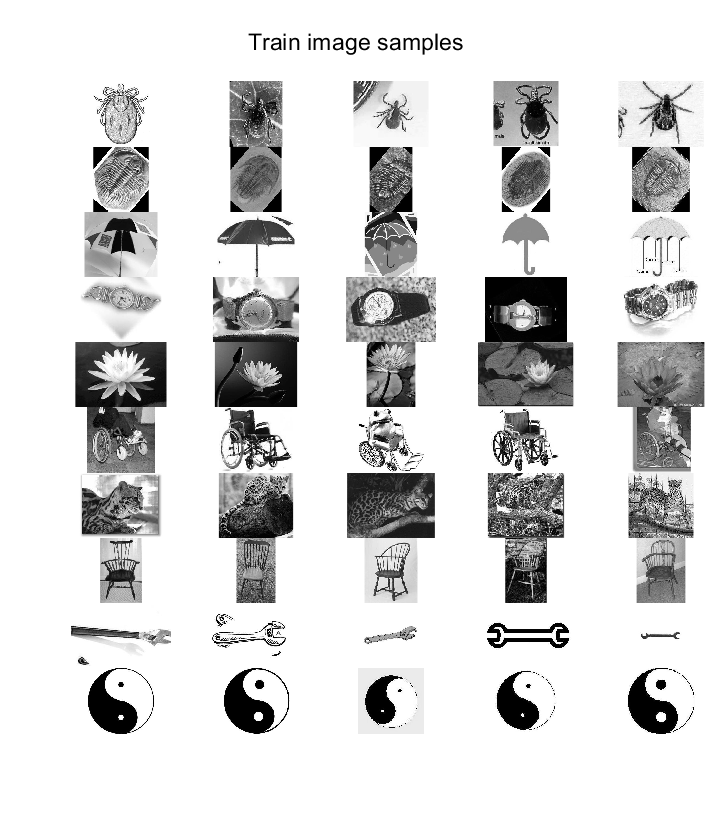
\includegraphics[height=6cm]{image/q1-appendix/train_img.png} 
		\caption{Train image samples}
	\end{subfigure}%
	\hfill
	\begin{subfigure}[t]{0.3\linewidth}
		\centering
		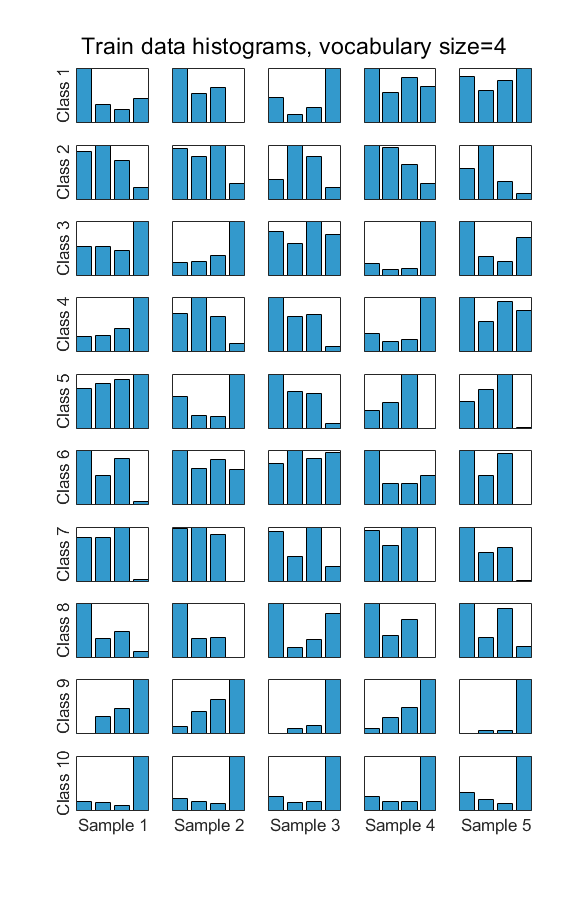
\includegraphics[height=6cm]{image/q1-appendix/train_4.png}
		\caption{Train data quantisation result, $K=4$}
	\end{subfigure}
	\hfill
	\begin{subfigure}[t]{0.3\linewidth}
		\centering
		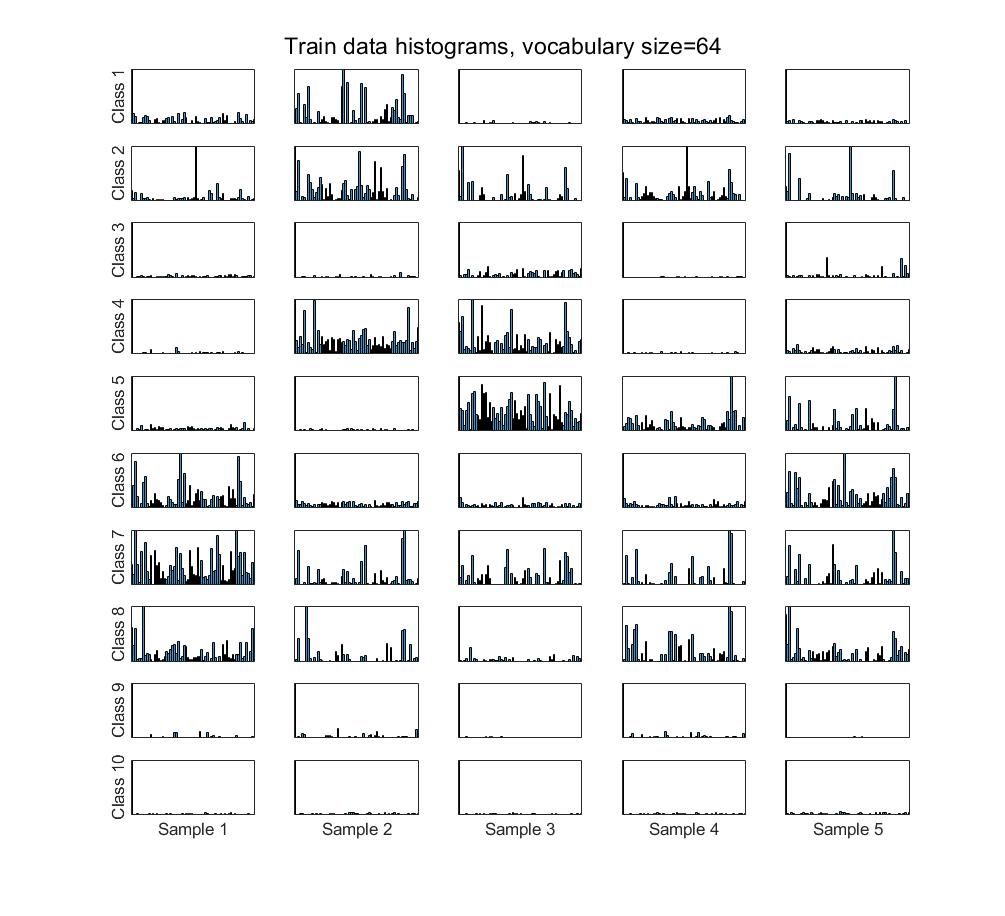
\includegraphics[height=6cm]{image/q1-appendix/train_64.png}
		\caption{Train data quantisation result, $K=64$}
	\end{subfigure}
	\caption{Visualistaion of train data quantisation result}
	\label{fig:q1_histogram_tr}
\end{figure}

\begin{figure}[htbp]
	\centering
	\begin{subfigure}[t]{0.3\linewidth}
		\centering
		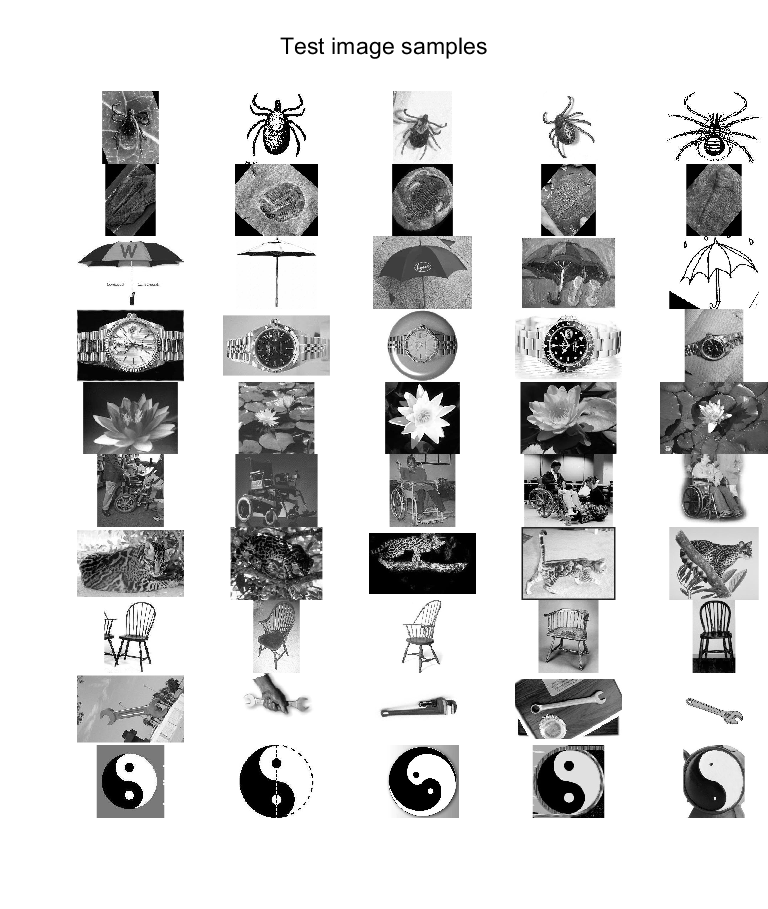
\includegraphics[height=6cm]{image/q1-appendix/test_img.png} 
		\caption{Test image samples}
	\end{subfigure}%
	\hfill
	\begin{subfigure}[t]{0.3\linewidth}
		\centering
		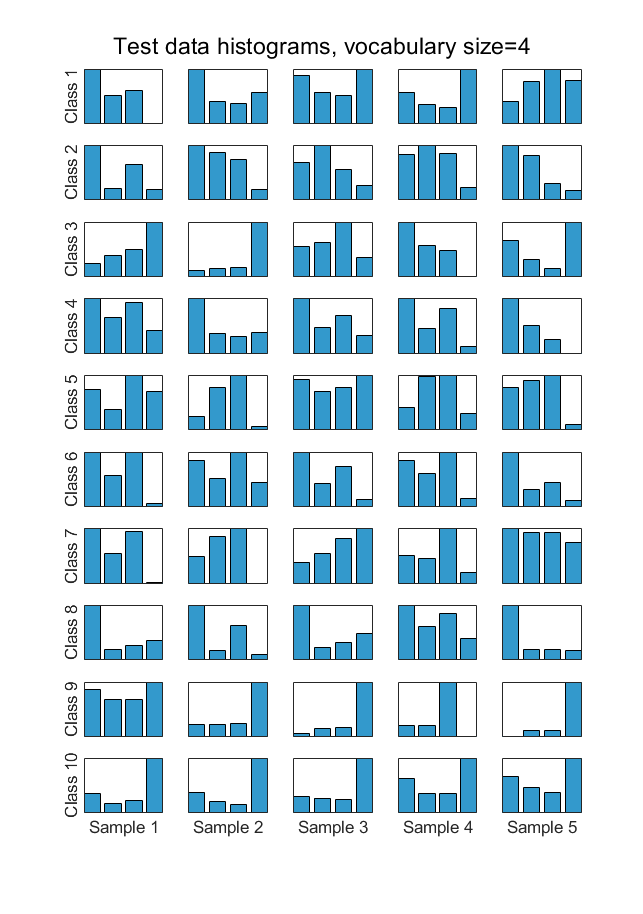
\includegraphics[height=6cm]{image/q1-appendix/test_4.png}
		\caption{Test data quantisation result, $K=4$}
	\end{subfigure}
	\hfill
	\begin{subfigure}[t]{0.3\linewidth}
		\centering
		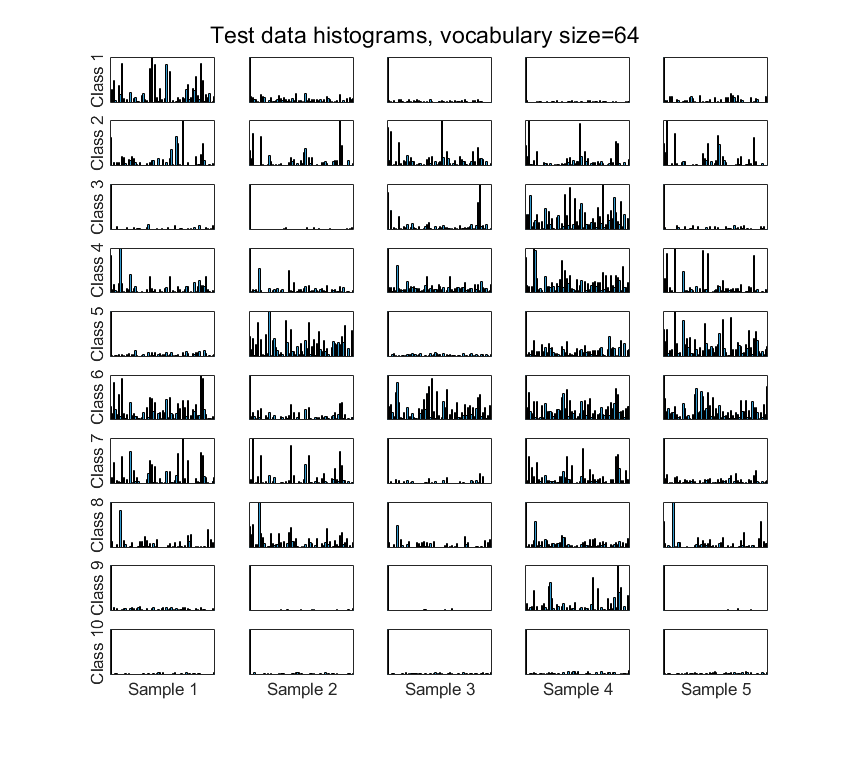
\includegraphics[height=6cm]{image/q1-appendix/test_64.png}
		\caption{Test data quantisation result, $K=64$}
	\end{subfigure}
	\caption{Visualistaion of test data quantisation result}
	\label{fig:q1_histogram_te}
\end{figure}

\section{Q1:Cosine similarity between images in \cref{fig:q1-fig2}}
\label{subsec:Q1_cossim}
\begin{figure}[htbp]
	\centering
	\begin{subfigure}[t]{0.25\linewidth}
		\centering
		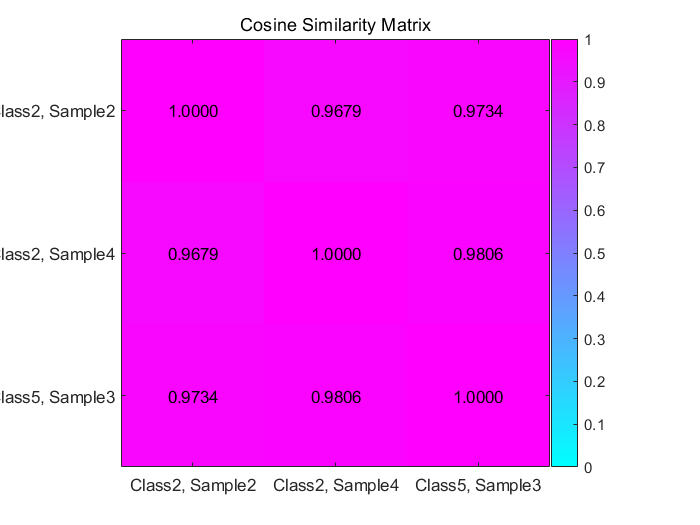
\includegraphics[width=\linewidth]{image/q1-appendix/similarity_4.png} 
		\caption{$K=4$}
	\end{subfigure}%
	\hfill
	\begin{subfigure}[t]{0.25\linewidth}
		\centering
		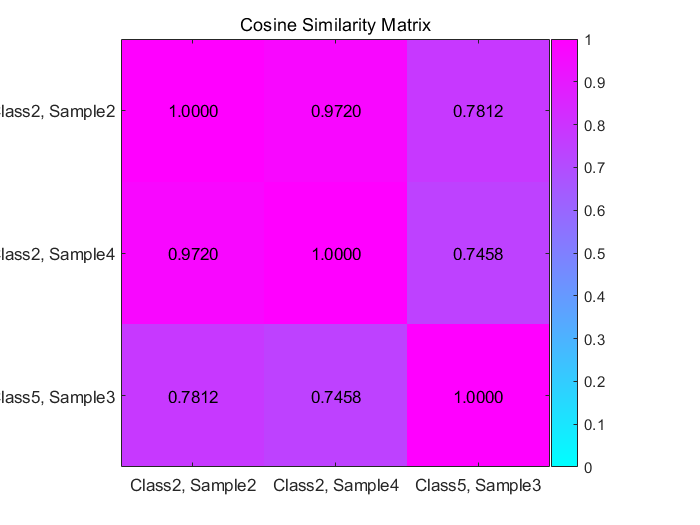
\includegraphics[width=\linewidth]{image/q1-appendix/similarity_16.png} 
		\caption{$K=16$}
	\end{subfigure}%
	\hfill
	\begin{subfigure}[t]{0.25\linewidth}
		\centering
		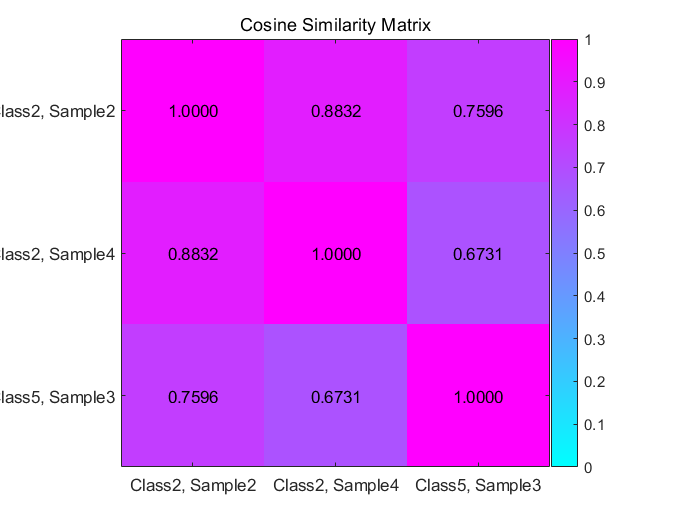
\includegraphics[width=\linewidth]{image/q1-appendix/similarity_64.png} 
		\caption{$K=64$}
	\end{subfigure}%
	\hfill
	\begin{subfigure}[t]{0.25\linewidth}
		\centering
		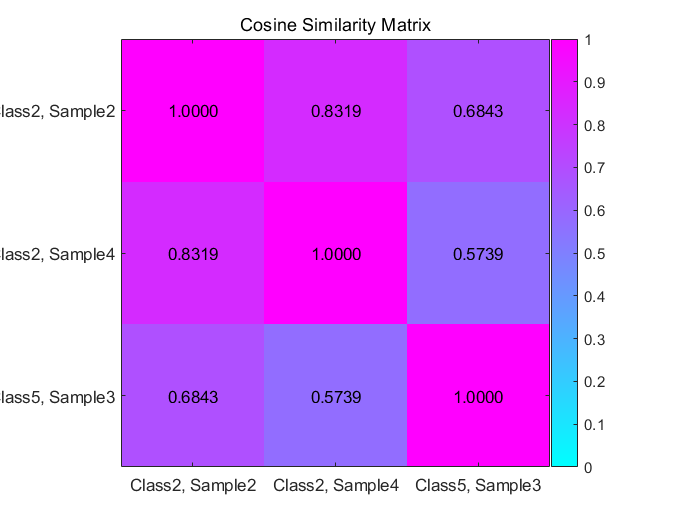
\includegraphics[width=\linewidth]{image/q1-appendix/similarity_256.png} 
		\caption{$K=256$}
	\end{subfigure}%
	\caption{Visualization of cosine similarity matrix of \cref{fig:q1-fig2} according to the different $K$}
	\label{fig:q1_cossim}
\end{figure}

\section{Q2: Test result's confusion matrix and success/failure cases}
\label{subsec:Q2-app1}

\section{Q2: Visualization of random forest's information gain process}
\label{subsec:Q2-app2}
